\documentclass[a4paper]{report}
\usepackage[utf8]{inputenc}
\usepackage[T1]{fontenc}
\usepackage{RJournal}
\usepackage{amsmath,amssymb,array}
\usepackage{booktabs}


% tightlist command for lists without linebreak
\providecommand{\tightlist}{%
  \setlength{\itemsep}{0pt}\setlength{\parskip}{0pt}}

\usepackage{longtable}

% Always define CSL refs as bib entries are contained in separate doc
% Pandoc citation processing
\newlength{\cslhangindent}
\setlength{\cslhangindent}{1.5em}
\newlength{\csllabelwidth}
\setlength{\csllabelwidth}{3em}
\newlength{\cslentryspacingunit} % times entry-spacing
\setlength{\cslentryspacingunit}{\parskip}
% for Pandoc 2.8 to 2.10.1
\newenvironment{cslreferences}%
  {}%
  {\par}
% For Pandoc 2.11+
\newenvironment{CSLReferences}[2] % #1 hanging-ident, #2 entry spacing
 {% don't indent paragraphs
  \setlength{\parindent}{0pt}
  % turn on hanging indent if param 1 is 1
  \ifodd #1
  \let\oldpar\par
  \def\par{\hangindent=\cslhangindent\oldpar}
  \fi
  % set entry spacing
  \setlength{\parskip}{#2\cslentryspacingunit}
 }%
 {}
\usepackage{calc}
\newcommand{\CSLBlock}[1]{#1\hfill\break}
\newcommand{\CSLLeftMargin}[1]{\parbox[t]{\csllabelwidth}{#1}}
\newcommand{\CSLRightInline}[1]{\parbox[t]{\linewidth - \csllabelwidth}{#1}\break}
\newcommand{\CSLIndent}[1]{\hspace{\cslhangindent}#1}



\begin{document}


%% do not edit, for illustration only
\sectionhead{Contributed research article}
\volume{15}
\volnumber{2}
\year{2023}
\month{June}
\setcounter{page}{25}

\begin{article}
  % !TeX root = RJwrapper.tex
\title{hydrotoolbox, a Package for Hydrometeorological Data Management}


\author{by Ezequiel Toum and Pierre Pitte}

\maketitle

\abstract{%
The hydrometeorological data provided by federal agencies, research groups and private companies tend to be heterogeneous: records are kept in different formats, quality control processes are not standardized and may even vary within a given agency, variables are not always recorded with the same temporal resolution, and there are data gaps and incorrectly recorded values. Once these problems are dealt with, it is useful to have tools to safely store and manipulate the series, providing temporal aggregation, interactive visualization for analysis, static graphics to publish and/or communicate results, techniques to correct and/or modify the series, among others. Here we introduce a package written in the R language using object-oriented programming and designed to accomplish these objectives, giving to the user a general framework for working with any kind of hydrometeorological series. We present the package design, its strengths, limitations and show its application for two real cases.
}

\hypertarget{introduction}{%
\section{Introduction}\label{introduction}}

Data management has generated growing interest among the scientific community
(Venkatraman 2013; Donoho 2017), driven by the proliferation of
data sharing through the internet, new
measurement techniques and equipment, and open and free access to
information obtained from remote sensing. It is also fueled by new and
growing demands from agencies and governments (national and/or regional)
for data-informed decision-making. To realize the full potential of
the available information, there is a need for accurate and efficient
tools that can pre-process these vast and heterogeneous data into more
convenient data sets (Addor et al. 2020).\\
The hydrological community uses data from hydrometeorological stations,
remote sensing observations and outputs from climatic and/or
hydrological models (Beven 2012). These data types may include (but
are not limited to):

\begin{enumerate}
\def\labelenumi{\alph{enumi}.}
\item
  \textbf{remote sensing}: snow cover images, soil humidity, glacier cover
  areas, digital elevation models.
\item
  \textbf{hydro-met stations}: air temperature, relative humidity, incoming
  solar radiation, atmospheric pressure, precipitation, streamflow
  records.
\item
  \textbf{numerical weather models}: air temperature, precipitation, and
  wind speed forecasting.
\item
  \textbf{hydrological models}: evolution of the snowpack, simulated
  streamflow, infiltration rates.
\item
  \textbf{large-sample hydrology datasets}
\end{enumerate}

\noindent
Data from remote sensing and climate models is distributed in
standardized formats (e.g., \emph{.nc}, \emph{.tiff}, \emph{.grb}) and therefore there
are standardized tools to manipulate them (Hijmans 2017; Conrad et al. 2015; Pierce 2019). This is not the case for hydrometeorological data as each
agency, research group or private company has its own standards.
Therefore, the formats, publication frequency, temporal resolution and
quality control vary. As an example, in Argentina, the
organizations that manage hydrological data tend to use proprietary software:
a) the \emph{Autoridad Interjurisdiccional de las Cuencas de los ríos Limay, Neuquén}
\emph{y Negro} (AIC) uses DIMS (Dynamic Integrated Monitoring System), b) the
\emph{Sistema Nacional de Información Hídrica} (SNIH) works with Mnemos, and
c) the \emph{Instituto Nacional del Agua} (INA) uses their own software
(personal communication).

The R language has gained a central role within the hydrological
community during the last decade because it allows the user to: a)
download and work with multiple data types and formats, b) extract,
manipulate and order data, c) develop hydrological models, d) conduct
statistical analyses, e) view results, and f) export images and
documents ready for publication. Slater et al. (2019) pointed out the
benefits and advantages of using R in the hydrological
field: (1) it democratizes science and numerical literacy; (2) it helps
the research to be reproducible and open; (3) provides statistical
tools; (4) allows connection to and from other languages; and (5) has
the support from a constantly growing community. Indeed the R
community has developed many packages for managing hydrological data
(\url{https://cran.r-project.org/web/views/Hydrology.html}), but they tend
to be either focused on Europe and North America or lack a
general-purpose framework for efficiently and safely storing and manipulating
hydrometeorological series:

\begin{enumerate}
\def\labelenumi{\arabic{enumi}.}
\item
  \textbf{hddtools} (Vitolo 2017): is designed to facilitate
  access to a variety of online open data sources relevant for
  hydrologists and, more generally, environmental scientists and
  practitioners. It includes functionality for Koppen Climate
  Classification, Global Runoff Data Centre, Data60UK, MOPEX (USA) and
  SEPA (Scotland).
\item
  \textbf{climate} (Czernecki, Głogowski, and Nowosad 2020): allows automatic downloading
  of OGIMET, University of Wyoming (atmospheric vertical profiling
  data), Polish Institute of Meteorology and Water Management
  (National Research Institute) and National Oceanic \& Atmospheric
  Administration (NOAA).
\item
  \CRANpkg{waterData} (Ryberg and Vecchia 2017): imports U.S. Geological
  Survey (USGS) daily hydrologic data from USGS web services, plots
  the data, addresses some common data problems, calculates and plots
  anomalies.
\item
  \CRANpkg{hydroTSM} (Zambrano-Bigiarini 2020): provides functions for
  management, analysis, interpolation and plotting of time series used
  in hydrology and related environmental sciences. This package is
  highly oriented towards hydrological modeling tasks.
\item
  \CRANpkg{dataRetrieval} (De Cicco et al. 2018): is a collection of
  functions that help to retrieve U.S. Geological Survey (USGS) and U.S.
  Environmental Protection Agency (EPA) water quality and hydrology
  data from web services.
\item
  \CRANpkg{hyfo} (Xu 2020): is a package with focus on
  processing and visualization of hydrological data and
  climate forecasting.
  Main function includes data extraction, data downscaling,
  resampling, gap filler of precipitation, bias correction of
  forecasting data, flexible time series plot, and spatial map
  generation.
\end{enumerate}

\CRANpkg{hydrotoolbox} (Toum 2022) is an R package developed
using R's object-oriented programming system (S4 classes; Chambers (2017)) that
provides a general framework for efficiently storing and manipulating multiple
hydrometeorological datasets, exploiting not only S4 advantages but
base R's copy on modify semantics. The series and its metadata (e.g.:
geo-referenced location, river basin name, country, among others) are
agglomerated in a single class object, allowing for an effective management
of vast and heterogeneous hydrometeorological data.
\pkg{hydrotoolbox} also provides a general set of methods regarding: a)
reading multiple datasets with their unique data formats (i.e.
delimited files such as comma-separated values (CSV) and tab-separated
values (TSV) and excel files), b) static and interactive time-series
plotting, c) data manipulation, d) data temporal aggregation, among
others. In addition, the current version (v 1.1.2) has specific
functions for reading data from Argentina and Chile. Despite this fact,
we want to stress that every user can combine other R functions or
packages for downloading and reading data (including those coming from
large-sample hydrological datasets; Addor et al. (2020)) with the
functionality of the package.

The rest of this work is organized as follows:
in the \textbf{Package design} section we
describe the underlying ideas with a brief description of the
classes, subclasses, methods and functions that \pkg{hydrotoolbox}
offers. In the \textbf{Case studies section} we show two applied
examples: the first deals with a hydrometerological data set and the second
deals with post-processing the results of a modeling exercise with the
\CRANpkg{HBV.IANIGLA} model (Toum 2021; Toum et al. 2021). These cases
lead to discussion about the package performance. We conclude with a
discussion of possible improvements and ways to extend the functionality
\pkg{hydrotoolbox}.

\hypertarget{package-design}{%
\section{Package design}\label{package-design}}

\pkg{hydrotoolbox} uses the object-oriented programming (OOP) paradigm,
a feature that makes the package flexible and allows other programmers
to extend its functionality. In this package, the properties are related to the
hydrometeorological variables and the methods with functions for
these objects manipulation. The following principles guided the
design of \pkg{hydrotoolbox}:

\begin{enumerate}
\def\labelenumi{\arabic{enumi}.}
\item
  \textbf{The time series of each variable must be grouped into stations},
  as they are organized based on their geographic location. This allows
  series registered in the same station or at different ones to be
  compared without losing their position, a fundamental aspect for a
  correct physical interpretation of the data.
\item
  \textbf{Modifications must be recorded in the same file}. Most time
  series have errors that need to be corrected. This could happen
  because the time series are discontinuous, the instruments fail, the
  variables are not all measured in the same temporal resolution,
  because of power cuts, or because local natural conditions
  induce erroneous measurements (e.g., snowfall undercatch
  due to wind; Goodinson and Louie (1998)). Errors are corrected in successive
  steps but it is crucial to have access to all versions of the
  series. This principle also seeks to avoid having multiple records
  of the same variable in a given station. The reader will find
  an example in the \emph{Case studies} section.
\item
  \textbf{Expedited visualization}. Fast and flexible visualization
  techniques are a powerful tool for analyzing and communicating results.
  The series should be able to be viewed statically and dynamically.
\item
  \textbf{There should be general functions for data manipulation} to
  reduce the need to permanently create custom functions.
\item
  \textbf{Open-ended design} to incorporate new objects and/or methods to
  continue expanding the package's functionality.
\end{enumerate}

\hypertarget{classes-and-subclasses}{%
\subsection{Classes and subclasses}\label{classes-and-subclasses}}

Following the first design principle, there is a class and two
subclasses for managing hydrometereological data (Figure \ref{fig:class-htb}).
The class, called \texttt{hydromet},
contains the station's metadata (e.g., geographic coordinates, name of
the basin, province, country, unique identifier, etc.). The two
subclasses correspond to \textbf{(a)} data from meteorological stations and
\textbf{(b)} data derived from modeling. The \texttt{hydromet\_station} subclass
contains a table for each measured variable (some of them are shown in
Table
\ref{tab:table-variables-static})
in combination with the metadata, allowing users to store in a single
object all the information concerning an hydrometeorological station.

\begin{figure}

{\centering 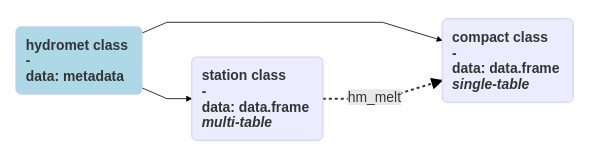
\includegraphics[width=0.7\linewidth]{./flow_diagram_classes_crop} 

}

\caption{Classes for hydrometeorological data in $\textbf{hydrotoolbox}$ package. Arrows indicate the class that each entity inherits from. The dotted arrow means that an $\texttt{hydromet\_station}$ class can be transformed (by the $\texttt{hm\_melt}$ method) to a  $\texttt{hydromet\_compact}$ class object.}\label{fig:class-htb}
\end{figure}

\noindent 
The remaining subclass, called \texttt{hydromet\_compact}, stores all
series in a single table (called \texttt{compact}). It was created so that
users could store input/output data from models or to save the same
variable to perform regional analyzes (e.g., precipitation series
recorded in different rain gauges).

\begin{table}

\caption{\label{tab:table-variables-static}Eight out of forty hydrometeorological variables supported in \texttt{hydromet\_station} class (use \texttt{slotNames(x = "hydromet\_station")} to see all of them). In the package most of them are rectangular tables containing date series in their first column (\texttt{Date} and \texttt{POSIX*} classes are allowed).}
\centering
\fontsize{9}{11}\selectfont
\begin{tabular}[t]{ll}
\toprule
\textbf{Slot} & \textbf{Variable}\\
\midrule
hq & water-height vs stream-discharge measurements\\
hw & water height level records\\
qh & hourly mean river discharge\\
qd & daily mean river discharge\\
qm & monthly mean river discharge\\
\addlinespace
qa & annual river discharge\\
wspd & wind speed\\
wdir & wind direction\\
. & \vphantom{2} .\\
. & \vphantom{1} .\\
\addlinespace
. & .\\
\bottomrule
\end{tabular}
\end{table}

\hypertarget{methods}{%
\subsection{Methods}\label{methods}}

The present package's version provides a set of data processing
operations (methods) widely required in hydrology such as: temporal
aggregation, interactive and static visualization, series modification and
statistical summaries. Table
\ref{tab:table-methods-static}
provides a complete list accompanied with a brief description. Also, to
make the package more user-friendly, all the methods for object
manipulation follow the syntax \texttt{hm\_action}; the \texttt{hm\_} prefix being
indicative of the superclass (\texttt{hydromet}) and the action being
indicative of what it does. We believe that this feature greatly eases
its application.

\begin{table}

\caption{\label{tab:table-methods-static}Processing operations for object manipulation in the \pkg{hydrotoolbox} package.}
\centering
\fontsize{9}{11}\selectfont
\begin{tabular}[t]{>{}ll}
\toprule
\textbf{Method} & \textbf{Description}\\
\midrule
\texttt{hm\_agg} & temporally aggregates  data\\
\texttt{hm\_build\_generic} & automatically loads raw data inside the \texttt{hydromet\_station} object\\
\texttt{hm\_create} & constructs the \texttt{hydromet} class and its subclasses\\
\texttt{hm\_get} & extracts the required table (or metadata) from the object\\
\texttt{hm\_melt} & merges several tables into a single one and set it into a \texttt{hydromet\_compact} class object\\
\addlinespace
\texttt{hm\_mutate} & creates, modifies and deletes columns inside an object table (slot)\\
\texttt{hm\_name} & changes data frame column names\\
\texttt{hm\_plot} & makes static and interactive graphs of the required hydrometeorological variables\\
\texttt{hm\_report} & gets basic statistic and a table with missing data\\
\texttt{hm\_set} & assigns the (meta)data to an \texttt{hydromet} class or subclass object\\
\addlinespace
\texttt{hm\_show} & shows the head or tail of the tables inside the object\\
\texttt{hm\_subset} & subsets the required table\\
\bottomrule
\end{tabular}
\end{table}

Although more details and examples about each of the methods are given
in the \textbf{Case studies} section and in the package documentation and
vignettes (Toum 2022), in the next lines we explain the use of \texttt{hm\_build\_generic}.
This is a core package function, since it allows to automatically
load raw hydrometeorological data inside an \texttt{hydromet\_station} class
object. Figure \ref{fig:read-like} depicts five different
compatible rectangular data configurations. The upper scheme shows
allowed configurations for any delimited type file (Wickham, Hester, and Bryan 2022): a)
all time series are stored in a single file with the first column being
the date and the others numeric time series (measured variables),
b) every variable is saved in a single file containing the date,
the time series and other kind of data (like data-quality flags).\\
Another widely used file type to store hydrometeorological measurements are
excel files. The bottom scheme of Figure \ref{fig:read-like} depicts the
three approaches: a) all time series are stored in a single file
and sheet, b) every sheet (all in the same file) contains a
variable (non-numeric columns allowed), and c) multiple files storing a
single variable.

\begin{figure}

{\centering 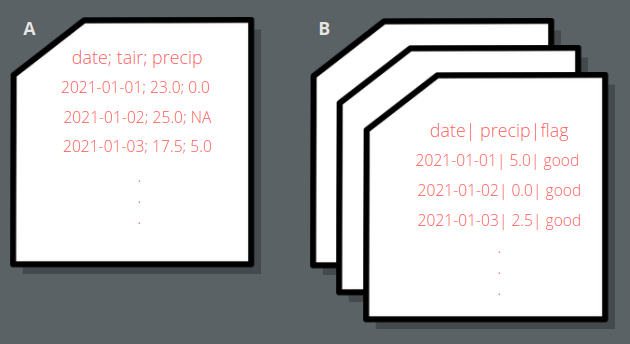
\includegraphics[width=0.52\linewidth]{./readr_like} 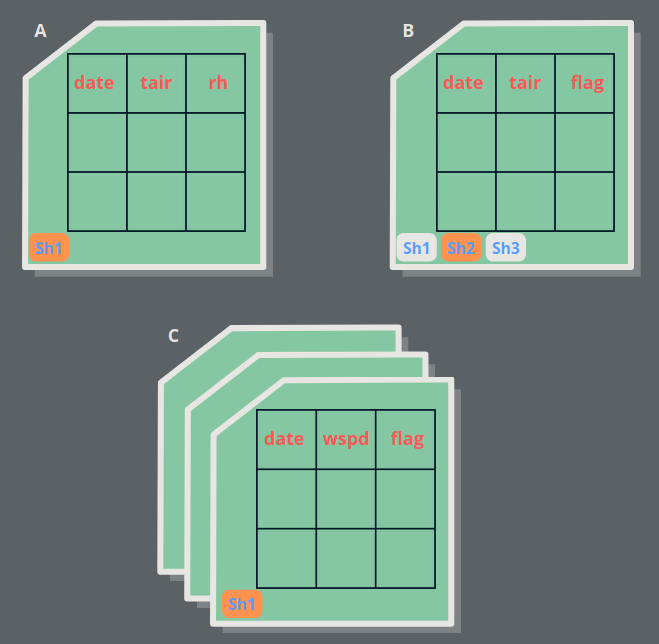
\includegraphics[width=0.52\linewidth]{./readxl_like} 

}

\caption{Rectangular data formats/file types compatible with the $\texttt{hm\_build\_generic}$ function. Top scheme depicts allowed delimited file arrangements while the bottom scheme is for excel files.}\label{fig:read-like}
\end{figure}

\noindent
The use of this function is illustrated with two examples (the data can be
downloaded from
\url{https://gitlab.com/ezetoum27/hydrotoolbox/-/tree/master/my_data}), but
the user can find full-covered documentation using the
\texttt{??hm\_build\_generic} command.

\begin{verbatim}
#* This code example shows how to use 
#* the hm_build_generic() method to 
#* automatically load raw hydrometeorological 
#* data

library(hydrotoolbox)
library(readr)
library(readxl)

# path to data
my_path <- "./home/my_folder/my_data"

#+++++++++++++++++++
# Rectangular data
#+++++++++++++++++++
#* Case B: multiple files (one per variable)
hm_create(class_name = "station") %>%
 hm_build_generic(path = my_path,
                  file_name = c("h_relativa_cuevas.csv",
                                "p_atm_cuevas.csv",
                                "precip_total_cuevas.csv",
                                "temp_aire_cuevas.csv",
                                "vel_viento_cuevas.csv"),
                  slot_name = c("rh", "patm", "precip",
                                "tair", "wspd"),
                  by = c("hour", "45 min", "30 min", "1 hour", "15 min"),
                  FUN = read_csv  ) %>%
 hm_show()


#+++++++++++++++++++
# Excel files
#+++++++++++++++++++
#* Case B: single file - multiple sheets (one per variable)
hm_create(class_name = "station") %>%
 hm_build_generic(path = my_path,
                  file_name = "mnemos_guido.xlsx",
                  slot_name = c("qd", "evap",
                                "tair","tmax",
                                "tmin"),
                  by = c(q = "day", evap =  "day",
                         tair = "6 hour", tmax = "day",
                         tmin = NULL),
                  FUN = read_excel,
                  sheet = c(1L:5L),
                  skip = 3,
                  out_name = list( c("q_m3/s", "flag"),
                                   c("evap_mm", "flag"),
                                   c("tair", "flag"),
                                   c("tmax", "flag"),
                                   c("tmin", "flag")
                  )
 ) %>%
 hm_show()
\end{verbatim}

\hypertarget{case-studies}{%
\section{Case studies}\label{case-studies}}

\hypertarget{daily-streamflow-record-at-the-guido-station-mendoza---argentina}{%
\subsection{Daily streamflow record at the Guido station (Mendoza - Argentina)}\label{daily-streamflow-record-at-the-guido-station-mendoza---argentina}}

The following example illustrates how to work with a time-series
recorded in an Excel file with a single sheet (Case \textbf{A} in the
\textbf{bottom} panel of Figure \ref{fig:read-like}). This variable is
measured at a station located in the Mendoza River basin from Argentina,
a watershed that covers an area of approximately \(7110 \, km^2\) and
provides water to almost \(1m\) inhabitants (Figure \ref{fig:mza-basin}).

\begin{figure}[h]

{\centering 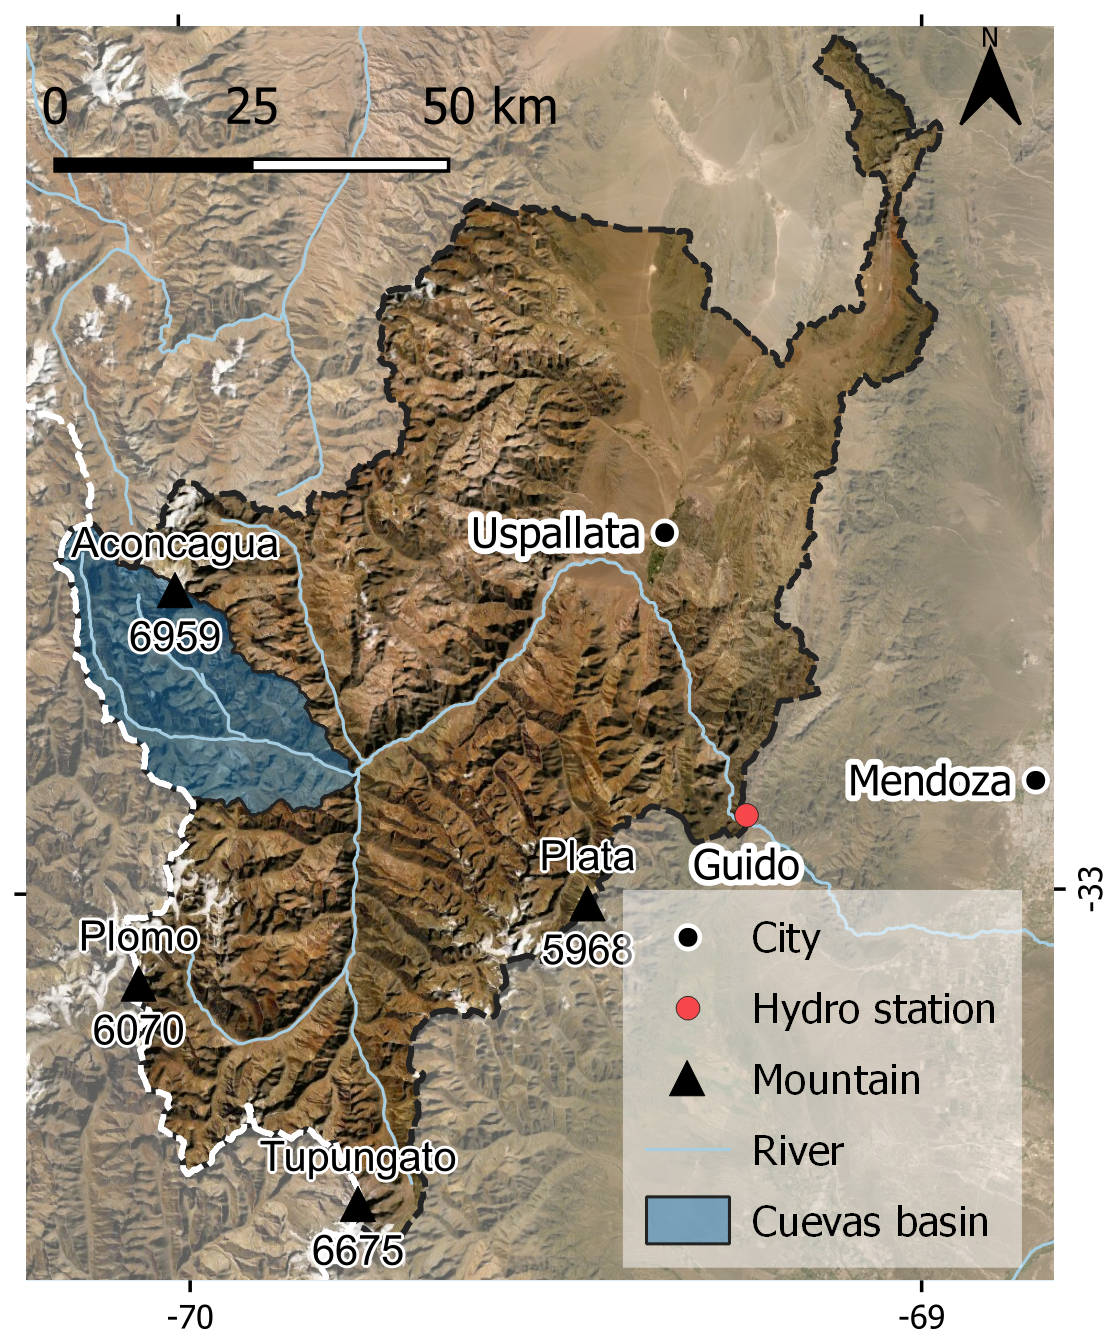
\includegraphics[width=0.6\linewidth]{./mza_basin} 

}

\caption{Map of the Mendoza basin including Guido hydrological station, cities, river and main mountain summits for reference.}\label{fig:mza-basin}
\end{figure}

In order to explore the data, we propose the following operations:

\begin{enumerate}
\def\labelenumi{\alph{enumi}.}
\item
  Build the station and obtain basic statistics of the data
  (\texttt{hm\_build\_generic}, \texttt{hm\_report} and \texttt{hm\_set} methods will be used).
\item
  Make a visual inspection of the series with \texttt{hm\_plot}.
\item
  Smooth the streamflow record using a five days moving average
  windows. \texttt{hm\_mutate} allows data manipulation and it can be combined
  with the user's or other package's functions via \texttt{FUN} and \texttt{...}
  arguments.
\item
  Aggregate the series to monthly average values (via \texttt{hm\_agg}).
\item
  Plot results for publishing using the \CRANpkg{ggplot2} (Wickham 2016)
  output of \texttt{hm\_plot}.
\end{enumerate}

\noindent 
The first step is to load the original data in a
\texttt{hydromet\_station} that we are going to called \emph{guido}.

\begin{verbatim}
library(hydrotoolbox)
library(readxl)

# package's data-base
path <- system.file("extdata", package = "hydrotoolbox")

# station building
guido <- 
  hm_create(class_name = "station") %>%
  hm_build_generic(path = path, 
                   file_name = "snih_qd_guido.xlsx", 
                   slot_name = "qd",
                   by = "1 day", 
                   out_name = list("q_m3/s"), 
                   sheet = 1L, 
                   FUN = read_excel)
\end{verbatim}

\noindent 
After executing these lines, the user will have an object that
contains a table (a \texttt{tibble} in this case) with the streamflow record in
the \texttt{qd} slot. When setting the argument \texttt{by\ =\ "1\ day"}, the function
automatically fill with \texttt{NA\_real\_} values the missing dates and also removes
duplicated records. On the other hand, using the default value (\texttt{by\ =\ NULL})
will ignore gaps, a feature that can be useful when loading
irregular time series.\\
As it was previously mentioned, the package also allows setting the
metadata inside the object. In this case we proposed to add the
basin area using \texttt{hm\_set}, but the user can apply the same command
to incorporate other information (see \texttt{??hm\_set}). Then \texttt{hm\_report}
is used to get basic statistics on the streamflow
record and also a table with a summary of the missing data. Note that this
function also contains the string
\texttt{"Missings\ total\ are\ in\ the\ last\ rows."}
(under \texttt{\$miss\_data\$comment}).

\begin{verbatim}
# set the basin area
guido <- 
  guido %>% 
  hm_set(basin_area = 7110)

# get streamflow's report
guido %>% 
  hm_report(slot_name = "qd")
\end{verbatim}

\begin{verbatim}
#> $stats
#>            date    q_m3/s
#> min  1956-07-01   8.00000
#> max  2020-06-30 401.00000
#> mean       <NA>  44.47951
#> sd         <NA>  36.53992
#> 
#> $miss_data
#> $miss_data$`q_m3/s`
#>        first       last time_steps
#> 1 1962-09-01 1962-09-30         30
#> 2 1970-02-13 1970-02-14          2
#> 3 1976-06-22 1976-07-31         40
#> 4 1985-06-01 1985-06-30         30
#> 5       <NA>       <NA>        102
#> 
#> $miss_data$comment
#> [1] "Missings total are in the last row."
\end{verbatim}

Another essential part of the workflow is data visualization
(Wickham and Grolemund 2017). The user of \pkg{hydrotoolbox} can use the \texttt{hm\_plot}
function and switch between static and interactive versions of the plot
(using the \texttt{interactive\ =\ TRUE} argument). Internally, this function
uses \pkg{ggplot2} and \CRANpkg{plotly} (Wickham 2016; Sievert 2020)
to reproduce time-series plots and provides several arguments to set
axes labels, define colors, line thickness
and type, transparency, among others. The following
example shows how to plot the mean daily streamflow. To see the interactive version
of Figure \ref{fig:guido-plot-static}
please visit the HTML (online) version of the article.

\begin{verbatim}
# ggplot2 daily flow
guido %>% 
  hm_plot(slot_name = "qd",
          col_name = list( "q_m3/s" ), 
          interactive = FALSE, 
          line_color = "dodgerblue",
          line_size = .7,
          y_lab = "Q(m3/s)", 
          from = "2010-07-01", 
          to = "2014-06-30") 
\end{verbatim}

\begin{figure}

{\centering 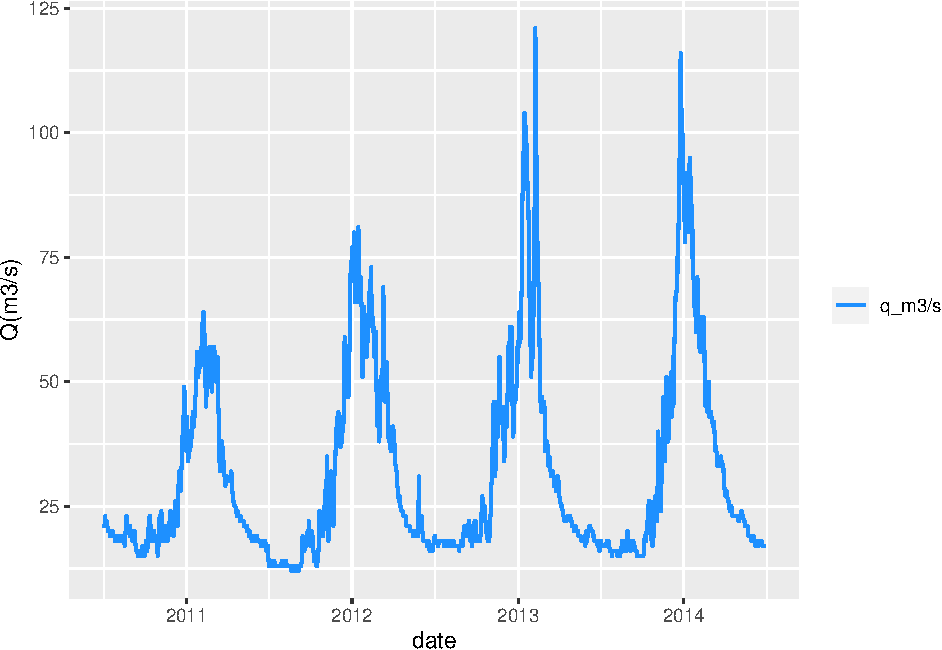
\includegraphics[width=1\linewidth]{RJ-2023-041_files/figure-latex/guido-plot-static-1} 

}

\caption{Plot of the Guido's streamflow time series (hydrologial years 2010/11 to 2013/14).}\label{fig:guido-plot-static}
\end{figure}

\begin{verbatim}
# plotly daily flow
guido %>% 
  hm_plot(slot_name = "qd",
          col_name = list( "q_m3/s" ), 
          interactive = TRUE, 
          line_color = "dodgerblue",
          line_size = .7,
          y_lab = "Q(m3/s)", 
          from = "2010-07-01",
          to = "2014-06-30") 
\end{verbatim}

As depicted in Figure \ref{fig:guido-plot-static} the time
series shows the effect of instrumental oscillations during the low water
flow periods.
One possible solution is to smooth the series using a moving average window.
To do this \pkg{hydrotoolbox} provides the \texttt{hm\_mutate}
method, a function that enable object's data manipulation. In this
example we combined the aforementioned method with the package's
function \texttt{roll\_fun}. Furthermore, in order to show another \texttt{hm\_mutate}
case, we removed two periods with records below a minimum
admissible value by setting them to \texttt{NA\_real\_}.

\begin{verbatim}
# smooth with roll_fun
guido <- 
  guido %>%
  hm_mutate(slot_name = "qd",
            FUN = roll_fun,
            col_name = "last",
            pos = "c",
            k = 5,
            mean,
            out_name = "q_smooth") 

# remove doubtful records with set_value
guido <- 
  guido %>%
  hm_mutate(slot_name = "qd",
            FUN = set_value,
            col_name = "q_smooth",
            out_name = "q_set",
            value = rep(NA_real_, 2),
            from = c("1965-08-09", "1974-06-26"),
            to = c("1965-08-25", "1974-07-04") )
\end{verbatim}

\noindent
After executing these expressions, the original and new series remain
stored in the same object. This feature avoids having multiple file
versions and allows to track the time series modifications,
achieving the second package's design principle
\emph{Modifications must be recorded in the same file}.

Moving forwards, the following code lines show how to temporally
aggregate this series at a monthly resolution via \texttt{hm\_agg} and how
to extract this new series and the basin area out of the
\emph{guido} object using \texttt{hm\_get}.

\begin{verbatim}
# aggregate daily mean streamflow 
# to mean monthly values
guido <- 
  guido %>%
  hm_agg(slot_name = "qd",
         col_name = "q_set", 
         fun = "mean", 
         period = "monthly", 
         out_name = "q_mean", 
         relocate = "qm", 
         allow_na = 2)

# extract the table 
tb_q_month <- 
  guido %>% 
  hm_get(slot_name = "qm")

# extract baisn area
basin_area <- 
  guido %>% 
  hm_get(slot_name = "basin_area")
\end{verbatim}

\noindent
In \texttt{hm\_agg} we allow a maximum of two missing daily discharge records
to compute the mean monthly streamflow and then, \texttt{hm\_get} extracts this
table so that the user may save and share it with others in \emph{CSV} format.
At this point is important to clarify that while \texttt{hm\_get} method extracts
any slot's data, the function \texttt{hm\_show} just prints the desired slot.

To conclude this first case study the monthly streamflow is
plotted (Figure \ref{fig:guido-ggplot}). As the \texttt{hm\_plot}
function generates a \texttt{ggplot2} object (when \texttt{interactive\ =\ FALSE})
the user can save and customize the graph to any style requirement.

\begin{verbatim}
# library
library(ggplot2)

# plot
gg_hm <-
  guido %>%
    hm_plot(slot_name = "qm", 
          col_name = list( c("q_mean") ), 
          line_color = "dodgerblue",
          line_size = .7,
          y_lab = "Q(m3/s)", x_lab = "", 
          legend_lab = "Mendoza River", 
          from = "1980-07-01", to = "1990-06-30") 
  
 # customize the graph
gg_out <- 
  gg_hm + 
    geom_point(col = "red", size = .8) +
    theme_light() + 
    scale_x_date( date_breaks = "4 month", date_labels = "%Y-%m" ) +
    scale_y_continuous(breaks = seq(0, 300, 50), limits = c(0, 300) ) +
    theme(axis.text = element_text(size = 8),
          axis.title.x = element_text(size = 10, face = "bold"),
          axis.text.x = element_text(angle = 90, vjust = 0.5),
          axis.title.y = element_text(size = 10, face = "bold"), 
          legend.position = "none")
        

gg_out
\end{verbatim}

\begin{figure}

{\centering 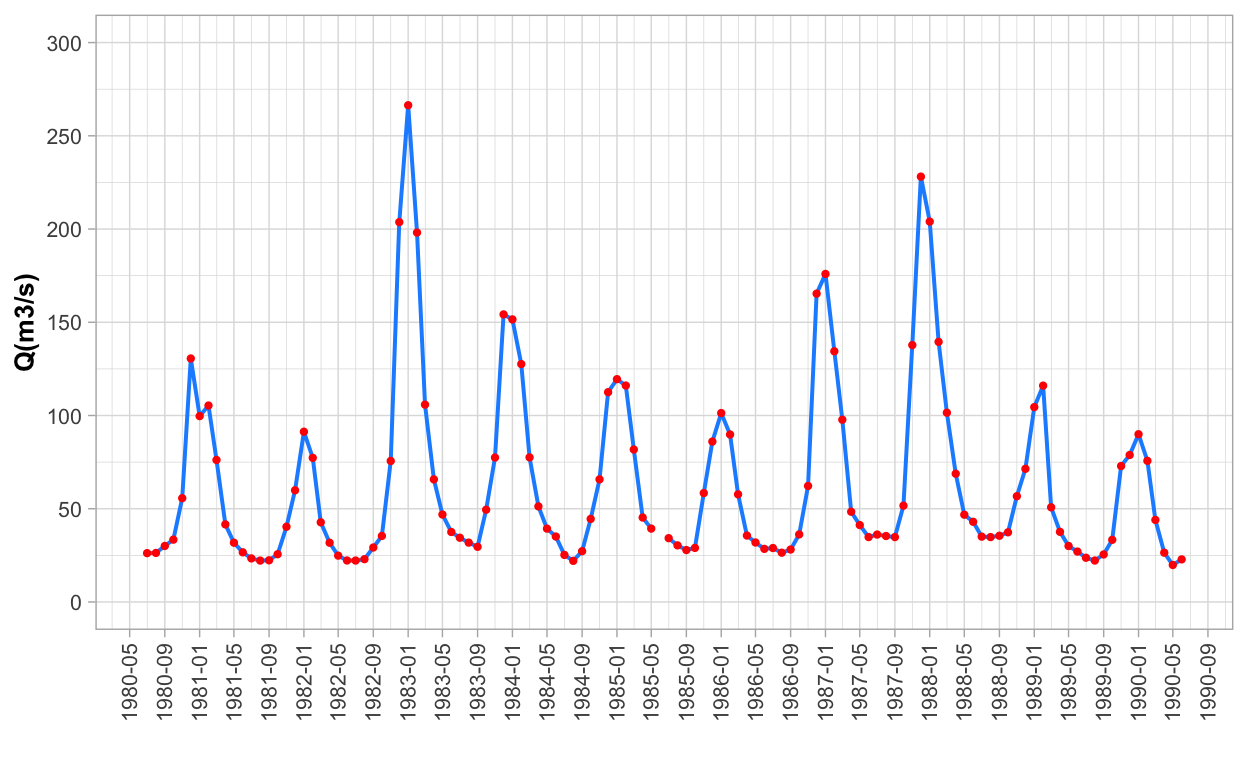
\includegraphics[width=1\linewidth]{RJ-2023-041_files/figure-latex/guido-ggplot-1} 

}

\caption{Example of customized time-series plot using the $\texttt{hm\_plot()}$ method in combination with labeling, scaling and theme options available on $\textbf{ggplot2}$.}\label{fig:guido-ggplot}
\end{figure}

\hypertarget{post-processing-of-the-hbv.ianigla-hydrological-model}{%
\subsection{Post processing of the HBV.IANIGLA hydrological model}\label{post-processing-of-the-hbv.ianigla-hydrological-model}}

The second case study shows how to use the package for post-processing a
numerical model output series. Specifically, it illustrates another
\texttt{hm\_mutate} case but in combination with another package function
(\texttt{mutate} from \CRANpkg{dplyr} package; Wickham et al. (2021)). The exercise
proposes to transform the units of the Cuevas River basin
(Figure \ref{fig:mza-basin}) glacier mass balance simulations
from \emph{millimeters of water equivalent} to \emph{meters of water equivalent}
and then plot it (Figure \ref{fig:cuevas-mb}). The
data for this example has been previously loaded into an
\texttt{hydromet\_compact} class object and the reader can download
the file from \url{https://gitlab.com/ezetoum27/hydrotoolbox/-/tree/master/my_data}).

\begin{verbatim}
# dplyr contains mutate()
library(dplyr) 

# glacier mass balance simulation
cuevas_mb <- readRDS(file = "data/cuevas_mb.rds" )

cuevas_mb <- 
  cuevas_mb %>%
  hm_mutate(slot_name = "compact",
            FUN = mutate, 
            `bm (m we)` = round( cuevas / 1000, 2 ),
            .keep = "all"
            ) 

cuevas_mb %>% hm_show()
\end{verbatim}

\begin{verbatim}
#> $compact
#>         date cuevas bm (m we)
#> 1 1981-04-01      0      0.00
#> 2 1982-04-01   1240      1.24
#> 3 1983-04-01    130      0.13
#> 4 1984-04-01    350      0.35
#> 5 1985-04-01    -80     -0.08
#> 6 1986-04-01    350      0.35
\end{verbatim}

\begin{verbatim}
# use hm_plot()
gg_out <- 
  cuevas_mb %>% 
  hm_plot(slot_name = "compact", 
          col_name = list("bm (m we)"), 
          line_color = "red3", 
          line_size = .7, 
          x_lab = "", y_lab = "MB (m we)"  )
  
# customize the figure
gg_out + 
geom_point(col = "blue", size = .8) +
  geom_hline(yintercept = 0) +
  theme_light() + 
  scale_x_date( date_breaks = "2 year", date_labels = "%Y" ) +
  scale_y_continuous(breaks = seq(-1.5, 1.5, 0.25),
                     limits = c(-1.5, 1.5) ) +
  theme(axis.text = element_text(size = 8),
        axis.title.x = element_text(size = 10, face = "bold"),
        axis.text.x = element_text(angle = 90, vjust = 0.5),
        axis.title.y = element_text(size = 10, face = "bold"), 
        legend.position = "none") 
\end{verbatim}

\begin{figure}

{\centering 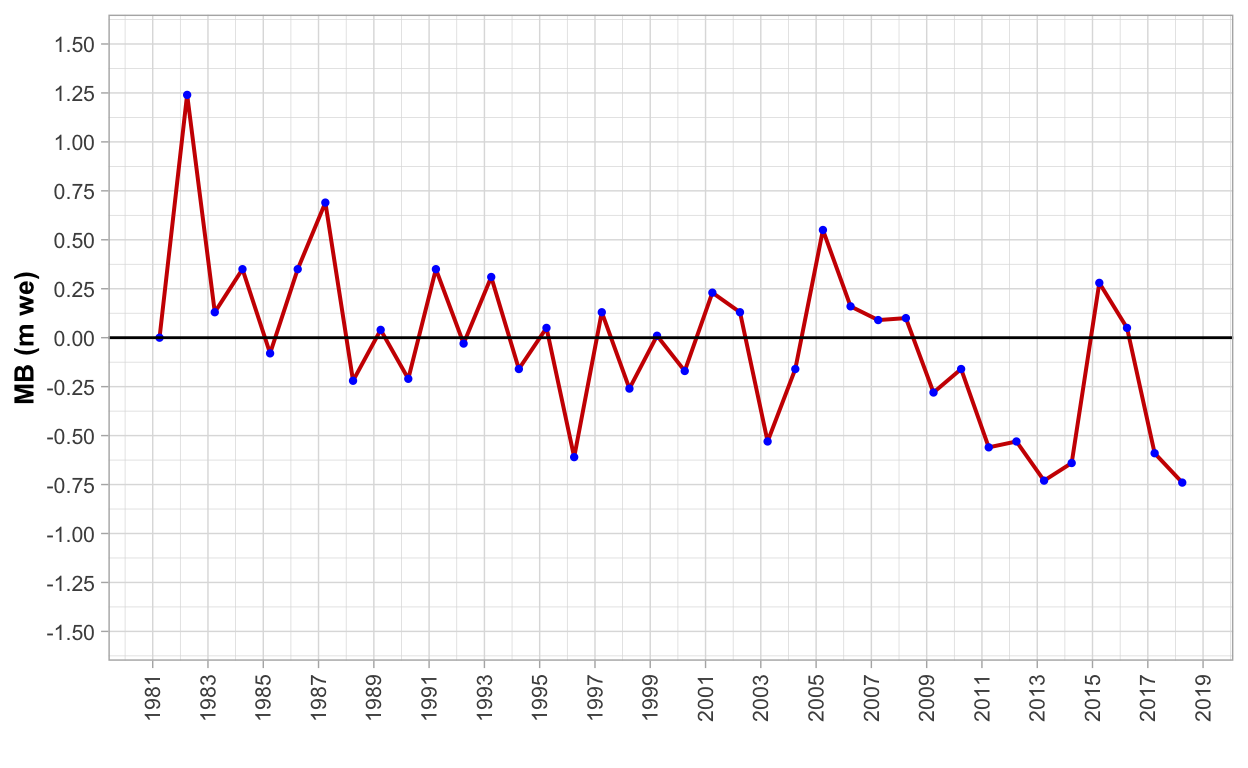
\includegraphics[width=1\linewidth]{RJ-2023-041_files/figure-latex/cuevas-mb-1} 

}

\caption{Model post-processing case example for the Cuevas basin annual glacier mass balance.}\label{fig:cuevas-mb}
\end{figure}

\noindent
This simple example suggests that \pkg{hydrotoolbox} is not only
suited for managing hydrometeorological series, but also for pre
and post processing hydrological modeling data.

\hypertarget{discussion}{%
\section{Discussion}\label{discussion}}

The R language community has made significant advances in the development
of hydrological packages, with many of them focusing on data access,
numerical modeling, and pre/post-processing (Slater et al. 2019). The new
\pkg{hydrotoolbox} package offers a general framework and methods for working with
hydrometeorological time series data management. To our knowledge, this
is the first general-purpose package for manipulating and visualizing
hydrometeorological data to this date.\\
In the literature there are at least two other packages available in the
CRAN repository that have some functionalities that could be considered
similar to \pkg{hydrotoolbox}, namely \pkg{hyfo} and \pkg{hydroTSM}
(Xu 2020; Zambrano-Bigiarini 2020). The first one was designed
as part of the European project EUPORIAS, and it is mainly focused
on data processing and visualization for hydrological and weather forecasting.
Therefore, this package's functions are specialized in spatial data
(e.g., NetCDF) in contrast to \pkg{hydrotoolbox} which focuses on
hydrometeorological stations recorded time series.
Additionally, \pkg{hyfo} uses \pkg{ggplot2} for visualization, which
can be used to create publication-quality static graphs but not interactive
visualizations. The other package, \pkg{hydroTSM}, is oriented towards tasks
related to modeling, a shared feature with \pkg{hydrotoolbox} but lacks
of a general-purpose system for hydrometeorological time series manipulation.
In programming terms, we think that object-oriented programming
(encapsulated or functional) is an essential mechanism for dealing with the
diversity of available data, while keeping things simpler for the user.
In addition, this paradigm makes \pkg{hydrotoolbox} robust in the following
aspects:

\begin{enumerate}
\def\labelenumi{\alph{enumi}.}
\item
  There are specific methods for manipulating and visualizing the objects
  that can be created with the package. This feature makes the workflow
  less prone to user error because specific and dedicated functions should
  be used to access the data.
\item
  The objects and the modifications that the user makes to the data time
  series are stored in the same object, avoiding the duplication of records
  that can occur in other datasets.
\item
  Once data has been incorporated, it is easy to get access and plot them.
  Additionally, \pkg{hydrotoolbox} allows saving the metadata which is a desirable
  feature when working with meteorological stations, data from numerical modeling, or
  series from large-sample hydrological datasets (Addor et al. 2020).
\end{enumerate}

\noindent 
Although \pkg{hyfo} and \pkg{hydroTSM} overlap with \pkg{hydrotoolbox}
in terms of numerical modeling and pre- and post-processing tasks,
neither of these two packages (or those mentionned previously) explicitly
cover hydrometeorological stations data management nor
provide a general working framework for this kind of records.

The package can be used in many applications and the user can also adapt
existing functions or packages with \pkg{hydrotoolbox}'s framework.
As case examples, the package's vignettes show how the \CRANpkg{tidyhydat}
(Albers 2017) and \textbf{weathercan} (LaZerte and Albers 2018) can be combined to work
with Canadian hydrometeorological records
(see \texttt{vignette(topic\ =\ "tidyhydat\_can",\ package\ =\ "hydrotoolbox")} and
\texttt{vignette(topic\ =\ "weathercan\_can",\ package\ =\ "hydrotoolbox")}).

In a recent publication, Addor et al. (2020) made a review of the current
state of large-sample hydrology (LSH) datasets. The authors proposed
general guidelines to support the creation of future LSH with some of
them listed here,

\begin{enumerate}
\def\labelenumi{\arabic{enumi}.}
\item
  \textbf{provide basic data for each basin}, with streamflow records being
  the cornerstone. The metadata should include the name, unique identifier,
  river and geographical coordinates of each streamgauge, catchment area
  and elevation info.\\
  \pkg{hydrotoolbox} provides all the objects with this metadata.
\item
  \textbf{following standards when naming variables}. Despite the fact that
  the package doesn't have the WATER ML-2
  (\url{https://www.ogc.org/standards/waterml} - last access 2022-10-13)
  variable names, the purpose of this feature is to ensure the
  consistency and comparability of environmental datasets.
  This R package provides with a description for each variable,
  allowing possible inter-dataset comparisons.
\item
  \textbf{use publicly available code for data processing}, making code
  for producing the LSH dataset available. This feature is important
  among free and open source software (FOSS).\\
  As a case example, the CAMELS dataset (Alvarez-Garreton et al. 2018; Addor et al. 2017) provides
  their users with a GitHub repository with code written in R
  (\url{https://github.com/naddor/camels}). Despite this, the repository
  contains a set of functions instead of a package that can be installed
  in many operating systems, with documented functions and reproducible
  examples. The specialized \pkg{hydrotoolbox} may provide a general framework
  to integrate this functions.
\end{enumerate}

Though there are similar and commonly used software in departments related
to the management of hydrometeorological data, they are closed-source
proprietary programs. \pkg{hydrotoolbox} is a FOSS, which
is a key feature not only from the research perspective but also
for hydrological
practice. Open source brings transparency to the decision-making
and hydrological design processes, and helps to save license money
in emerging countries (Hutton et al. 2016).

To conclude this discussion, some users may have used the
older \CRANpkg{hydroToolkit} package. This turned out to be an
early version of \pkg{hydrotoolbox} that we decided to reform after
using it in a large project. We realized that the original five
subclasses could be reduced to two, simplifying not only their use
but also improving their long-term maintainability. In addition, we decided
to improve several methods (e.g., time series visualization) that were
limited in functionality. Also, to elaborate the syntax of the functions,
methods and their arguments, we followed the suggestions of
\emph{The tidyverse style guide} document (Wickham 2023), adapting the package
to the new standards used within the community of R programmers.

\hypertarget{summary}{%
\section{Summary}\label{summary}}

\pkg{hydrotoolbox} is an new contribution to the R hydrological community,
as it is specifically designed for working with hydrometeorological
station records. The package allows the data to be viewed
interactively3 (\pkg{plotly}) or statically (\pkg{ggplot2}) using the same method
(\texttt{hm\_plot}),3 it also allows the use of functions from other packages or
created by the user via the \texttt{hm\_mutate} method.

The case studies show two examples with different aims: the first processed
a streamflow record and the second uses a numerical model output to
plot results. More complete and varied examples are in the documentation of the
package and in3 its vignettes (\texttt{vignette(package\ =\ "hydrotoolbox")}).

\pkg{hydrotoolbox} is designed to incorporate future improvements. One of them
could be functions for visualizing station's geographical position
(using the metadata) on an
interactive map, and perhaps to allow the user to plot and compare recorded
time series. This new function could use capabilities of the
\CRANpkg{leaflet} package, a JavaScript library for producing interactive maps.
The main class, \texttt{hydromet}, could also combine the functionality of
existing packages such as \CRANpkg{raster} (Hijmans 2017) or \CRANpkg{sf}
(Pebesma 2018) to include other kind of spatial data (e.g., catchment
boundary, soil types, gridded meteorological data, among others).
Finally, new classes and methods could be included for processing field data
from glacier mass balance studies, an activity closely related to the study
of the hydrological cycle in cold regions. This kind of improvements may
also make the package useful in other scientific communities such as glaciology.

\hypertarget{references}{%
\section*{References}\label{references}}
\addcontentsline{toc}{section}{References}

\hypertarget{refs}{}
\begin{CSLReferences}{1}{0}
\leavevmode\vadjust pre{\hypertarget{ref-addor:2020}{}}%
Addor, Nans, Hong X. Do, Camila Alvarez-Garreton, Gemma Coxon, Keirnan Fowler, and Pablo A. Mendoza. 2020. {``Large-Sample Hydrology: Recent Progress, Guidelines for New Datasets and Grand Challenges.''} \emph{Hydrological Sciences Journal} 65 (April): 712--25. \url{https://doi.org/10.1080/02626667.2019.1683182}.

\leavevmode\vadjust pre{\hypertarget{ref-addor:2017}{}}%
Addor, Nans, Andrew J. Newman, Naoki Mizukami, and Martyn P. Clark. 2017. {``The {CAMELS} Data Set: Catchment Attributes and Meteorology for Large-Sample Studies.''} \emph{Hydrology and Earth System Sciences} 21 (10): 5293--313. \url{https://doi.org/10.5194/hess-21-5293-2017}.

\leavevmode\vadjust pre{\hypertarget{ref-tidyhydat:2017}{}}%
Albers, Sam. 2017. {``Tidyhydat: Extract and Tidy Canadian Hydrometric Data.''} \emph{The Journal of Open Source Software} 2 (20). \url{https://doi.org/10.21105/joss.00511}.

\leavevmode\vadjust pre{\hypertarget{ref-camila:2018}{}}%
Alvarez-Garreton, Camila, Pablo A. Mendoza, Juan Pablo Boisier, Nans Addor, Mauricio Galleguillos, Mauricio Zambrano-Bigiarini, Antonio Lara, et al. 2018. {``The {CAMELS}-{CL} Dataset: Catchment Attributes and Meteorology for Large Sample Studies -- {Chile} Dataset.''} \emph{Hydrology and Earth System Sciences} 22 (11): 5817--46. https://doi.org/\url{https://doi.org/10.5194/hess-22-5817-2018}.

\leavevmode\vadjust pre{\hypertarget{ref-beven:2012}{}}%
Beven, Keith J. 2012. \emph{Rainfall - {Runoff} {Modelling}}. 2 edition. Chichester: Wiley.

\leavevmode\vadjust pre{\hypertarget{ref-chambers:2017}{}}%
Chambers, John M. 2017. \emph{Extending {R}}. CRC Press.

\leavevmode\vadjust pre{\hypertarget{ref-saga:2015}{}}%
Conrad, O., B. Bechtel, M. Bock, H. Dietrich, E. Fischer, L. Gerlitz, J. Wehberg, V. Wichmann, and J. Böhner. 2015. {``System for {Automated} {Geoscientific} {Analyses} ({SAGA}) v. 2.1.4.''} \emph{Geoscientific Model Development} 8 (7). https://doi.org/\url{https://doi.org/10.5194/gmd-8-1991-2015}.

\leavevmode\vadjust pre{\hypertarget{ref-climate:2020}{}}%
Czernecki, Bartosz, Arkadiusz Głogowski, and Jakub Nowosad. 2020. {``Climate: {An} {R} {Package} to {Access} {Free} {In}-{Situ} {Meteorological} and {Hydrological} {Datasets} {For} {Environmental} {Assessment}.''} \emph{Sustainability} 12 (1). \url{https://doi.org/10.3390/su12010394}.

\leavevmode\vadjust pre{\hypertarget{ref-cicco:2018}{}}%
De Cicco, Laura A., David Lorenz, Robert M. Hirsch, William Watkins, and Mike Johnson. 2018. \emph{dataRetrieval: R Packages for Discovering and Retrieving Water Data Available from u.s. Federal Hydrologic Web Services} (version 2.7.7). Reston, VA: U.S. Geological Survey; U.S. Geological Survey. \url{https://doi.org/10.5066/P9X4L3GE}.

\leavevmode\vadjust pre{\hypertarget{ref-donoho:2017}{}}%
Donoho, David. 2017. {``50 {Years} of {Data} {Science}.''} \emph{Journal of Computational and Graphical Statistics} 26 (4): 745--66. \url{https://doi.org/10.1080/10618600.2017.1384734}.

\leavevmode\vadjust pre{\hypertarget{ref-goodinson:1998}{}}%
Goodinson, and Louie. 1998. {``{WMO} {Solid} {Precipitation} {Measurement} {Intercomparison}.''} 67. WMO.

\leavevmode\vadjust pre{\hypertarget{ref-raster:2017}{}}%
Hijmans, Robert J. 2017. \emph{Raster: Geographic Data Analysis and Modeling}. \url{https://CRAN.R-project.org/package=raster}.

\leavevmode\vadjust pre{\hypertarget{ref-hutton:2016}{}}%
Hutton, Christopher, Thorsten Wagener, Jim Freer, Dawei Han, Chris Duffy, and Berit Arheimer. 2016. {``Most Computational Hydrology Is Not Reproducible, so Is It Really Science?''} \emph{Water Resources Research} 52 (10): 7548--55. \url{https://doi.org/10.1002/2016WR019285}.

\leavevmode\vadjust pre{\hypertarget{ref-weathercan:2018}{}}%
LaZerte, Stefanie E, and Sam Albers. 2018. {``{weathercan}: {D}ownload and Format Weather Data from Environment and Climate Change Canada.''} \emph{The Journal of Open Source Software} 3 (22): 571. \url{https://joss.theoj.org/papers/10.21105/joss.00571}.

\leavevmode\vadjust pre{\hypertarget{ref-sf:2018}{}}%
Pebesma, Edzer. 2018. {``{Simple Features for R: Standardized Support for Spatial Vector Data}.''} \emph{{The R Journal}} 10 (1): 439--46. \url{https://doi.org/10.32614/RJ-2018-009}.

\leavevmode\vadjust pre{\hypertarget{ref-netcdf:2019}{}}%
Pierce, David. 2019. \emph{Ncdf4: Interface to Unidata netCDF (Version 4 or Earlier) Format Data Files}. \url{https://CRAN.R-project.org/package=ncdf4}.

\leavevmode\vadjust pre{\hypertarget{ref-ryberg:2017}{}}%
Ryberg, Karen R., and Aldo V. Vecchia. 2017. \emph{waterData: Retrieval, Analysis, and Anomaly Calculation of Daily Hydrologic Time Series Data}. \url{https://CRAN.R-project.org/package=waterData}.

\leavevmode\vadjust pre{\hypertarget{ref-plotly_pkg}{}}%
Sievert, Carson. 2020. \emph{Interactive Web-Based Data Visualization with r, Plotly, and Shiny}. Chapman; Hall/CRC. \url{https://plotly-r.com}.

\leavevmode\vadjust pre{\hypertarget{ref-slater:2019}{}}%
Slater, Louise J., Guillaume Thirel, Shaun Harrigan, Olivier Delaigue, Alexander Hurley, Abdou Khouakhi, Ilaria Prodoscimi, Claudia Vitolo, and Katie Smith. 2019. {``Using {R} in Hydrology: A Review of Recent Developments and Future Directions.''} \emph{Hydrology and Earth System Sciences Discussions}, February, 1--33. https://doi.org/\url{https://doi.org/10.5194/hess-2019-50}.

\leavevmode\vadjust pre{\hypertarget{ref-toum:2021}{}}%
Toum, Ezequiel. 2021. \emph{{HBV.IANIGLA}: Modular Hydrological Model}. \url{https://CRAN.R-project.org/package=HBV.IANIGLA}.

\leavevmode\vadjust pre{\hypertarget{ref-htoolbox:2021}{}}%
---------. 2022. \emph{Hydrotoolbox: Hydrological Tools for Handling Hydro-Meteorological Data Records}. \url{https://CRAN.R-project.org/package=hydrotoolbox}.

\leavevmode\vadjust pre{\hypertarget{ref-toum-rj:2021}{}}%
Toum, Ezequiel, Mariano H. Masiokas, Ricardo Villalba, Pierre Pitte, and Lucas Ruiz. 2021. {``{The HBV.IANIGLA Hydrological Model}.''} \emph{{The R Journal}} 13 (1): 378--95. \url{https://doi.org/10.32614/RJ-2021-059}.

\leavevmode\vadjust pre{\hypertarget{ref-venkatraman:2013}{}}%
Venkatraman, Vijaysree. 2013. {``When {All} {Science} {Becomes} {Data} {Science}.''} \emph{Science {\textbar} AAAS}. \url{https://www.sciencemag.org/careers/2013/05/when-all-science-becomes-data-science}.

\leavevmode\vadjust pre{\hypertarget{ref-vitolo:2017}{}}%
Vitolo, Claudia. 2017. {``Hddtools: Hydrological Data Discovery Tools.''} \emph{The Journal of Open Source Software} 2 (9). \url{https://doi.org/10.21105/joss.00056}.

\leavevmode\vadjust pre{\hypertarget{ref-ggplot2_pkg}{}}%
Wickham, Hadley. 2016. \emph{Ggplot2: Elegant Graphics for Data Analysis}. Springer-Verlag New York. \url{https://ggplot2.tidyverse.org}.

\leavevmode\vadjust pre{\hypertarget{ref-tidystyle}{}}%
---------. 2023. \emph{The Tidyverse Style Guide}. \url{https://style.tidyverse.org/}.

\leavevmode\vadjust pre{\hypertarget{ref-dplyr:2021}{}}%
Wickham, Hadley, Romain François, Lionel Henry, and Kirill Müller. 2021. \emph{Dplyr: A Grammar of Data Manipulation}. \url{https://CRAN.R-project.org/package=dplyr}.

\leavevmode\vadjust pre{\hypertarget{ref-hadley_r_data}{}}%
Wickham, Hadley, and Garrett Grolemund. 2017. \emph{R for {Data} {Science}: {Import}, {Tidy}, {Transform}, {Visualize}, and {Model} {Data}}. Edición: 1. Sebastopol, CA: O'Reilly Media.

\leavevmode\vadjust pre{\hypertarget{ref-readr_pkg}{}}%
Wickham, Hadley, Jim Hester, and Jennifer Bryan. 2022. \emph{Readr: Read Rectangular Text Data}. \url{https://CRAN.R-project.org/package=readr}.

\leavevmode\vadjust pre{\hypertarget{ref-hyfo:2020}{}}%
Xu, Yuanchao. 2020. \emph{Hyfo: Hydrology and Climate Forecasting}. \url{https://CRAN.R-project.org/package=hyfo}.

\leavevmode\vadjust pre{\hypertarget{ref-zambrano:2020}{}}%
Zambrano-Bigiarini, Mauricio. 2020. \emph{hydroTSM: Time Series Management, Analysis and Interpolation for Hydrological Modelling}. \url{https://github.com/hzambran/hydroTSM}.

\end{CSLReferences}


\address{%
Ezequiel Toum\\
IANIGLA-CONICET\\%
Av. Ruiz Leal s/n Parque General San Martin - Mendoza\\ Argentina\\
%
%
\textit{ORCiD: \href{https://orcid.org/0000-0002-4482-0559}{0000-0002-4482-0559}}\\%
\href{mailto:etoum@mendoza-conicet.gob.ar}{\nolinkurl{etoum@mendoza-conicet.gob.ar}}%
}

\address{%
Pierre Pitte\\
IANIGLA-CONICET\\%
Av. Ruiz Leal s/n Parque General San Martin - Mendoza\\ Argentina\\
%
%
\textit{ORCiD: \href{https://orcid.org/0000-0001-5625-8287}{0000-0001-5625-8287}}\\%
\href{mailto:pierrepitte@mendoza-conicet.gob.ar}{\nolinkurl{pierrepitte@mendoza-conicet.gob.ar}}%
}

\end{article}


\end{document}
